% 
%            ,,                                        
%          `7MM            _.o9                                
%            MM                                             
%  ,6"Yb.    MM  ,p6"bo   ,6"Yb.  M"""MMV  ,6"Yb.  `7Mb,od8 
% 8)   MM    MM 6M'  OO  8)   MM  '  AMV  8)   MM    MM' "' 
%  ,pm9MM    MM 8M        ,pm9MM    AMV    ,pm9MM    MM     
% 8M   MM    MM YM.    , 8M   MM   AMV  , 8M   MM    MM     
% `Moo9^Yo..JMML.YMbmd'  `Moo9^Yo.AMMmmmM `Moo9^Yo..JMML.   
% 
% 
% Free and Open-Source template for academic works
% https://github.com/dpmj/alca



\section{Orchestrare carichi di lavoro}

Orchestrazione dei carichi di lavoro in ambito informatico si riferisce al processo di gestione, coordinamento e automazione delle attività e delle risorse coinvolte nell'esecuzione di applicazioni distribuite e complesse. Questa pratica è particolarmente rilevante nei contesti in cui le applicazioni sono composte da componenti modulari, come nel caso delle architetture a microservizi o in generale delle infrastrutture basate su container.

\subsection{Kubernetes}

L'analisi di Kubernetes richiede un approccio tecnico e preciso, considerando la complessità e l'ampiezza delle funzionalità che offre nell'orchestrazione e nella gestione dei container. Fondamentale è il contesto delle sue origini, risalenti al progetto Borg sviluppato in Google, il quale ha posto le basi per molte delle caratteristiche chiave di Kubernetes.

Kubernetes si basa su un modello dichiarativo, in cui gli utenti specificano lo stato desiderato dell'applicazione e il sistema si occupa di portare lo stato effettivo al corrispondente. Questo modello, ispirato dalla filosofia di Borg \cite{verma2015large}, consente la gestione semplificata e la scalabilità orizzontale degli applicativi distribuiti. Le risorse fisiche sono astratte e trattate come un pool omogeneo, garantendo una distribuzione efficiente dei container su nodi fisici o virtuali \cite{burns2016borg}.

Un elemento cruciale in Kubernetes è il concetto di Pod, che rappresenta la più piccola unità distribuibile. I Pod contengono uno o più container che condividono il medesimo contesto di rete e storage, semplificando la comunicazione e la condivisione delle risorse. Questo approccio consente di definire gruppi di container correlati, garantendo una coesione e una gestione semplificate \cite{burns2016borg}.

\begin{figure}[h]
    \centering
    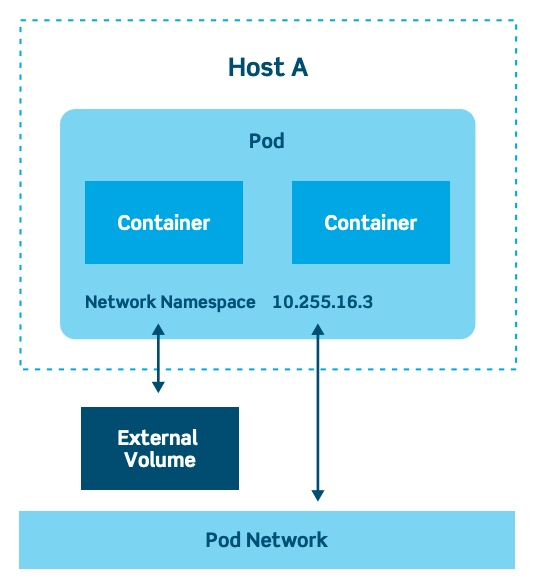
\includegraphics[width=300px]{figures/ch3/kube-pod.jpg}
    \caption[Overview ad alto livello di un pod]{Overview ad alto livello di un pod}
    \label{fig:cha3:k8s2}
\end{figure}

L'orchestrazione dei container è una delle funzionalità principali di Kubernetes. Il suo scheduler distribuisce i container su nodi disponibili, tenendo conto delle risorse richieste e delle politiche di allocazione definite. Questo processo, simile al sistema di scheduling di Borg \cite{burns2016borg}, contribuisce a una distribuzione efficiente dei carichi di lavoro su una vasta infrastruttura, garantendo una distribuzione bilanciata e affidabile \cite{burns2016borg}.

Un aspetto distintivo di Kubernetes è la sua capacità di garantire la disponibilità e la resilienza delle applicazioni attraverso i concetti di ReplicaSets e Servizi. ReplicaSets gestisce il numero desiderato di repliche di un Pod, assicurando che il sistema mantenga sempre la configurazione desiderata. I Servizi, ispirati al concetto di servizio di rete in Borg \cite{verma2015large}, forniscono un punto di accesso stabile per i Pod, garantendo la comunicazione affidabile all'interno del cluster \cite{burns2016borg}.

La gestione delle configurazioni e delle segrete è un aspetto critico di Kubernetes, che adotta il modello dichiarativo anche in questo contesto. Gli oggetti ConfigMap e Secret consentono la separazione tra la configurazione dell'applicazione e i dati sensibili, agevolando la gestione, l'aggiornamento e la distribuzione di configurazioni complesse \cite{hightower2017kubernetes}.

Infine, la flessibilità di Kubernetes è evidente nella sua capacità di estendere le funzionalità di base attraverso i Custom Resource Definitions (CRD) e gli Operator. Questi strumenti consentono agli sviluppatori di definire risorse personalizzate e le relative operazioni, adattando Kubernetes alle esigenze specifiche delle applicazioni \cite{burns2016borg}.

In conclusione, l'approfondimento tecnico di Kubernetes rivela una piattaforma estremamente sofisticata che deriva molte delle sue caratteristiche chiave dalle esperienze maturate con il progetto Borg in Google. L'orchestrazione, la gestione delle risorse, la disponibilità delle applicazioni e la flessibilità sono solo alcuni degli aspetti in cui Kubernetes eccelle, facendolo emergere come uno strumento fondamentale nell'ecosistema delle moderne architetture distribuite basate su container.

\subsubsection{Architettura di Kubernetes}

L'architettura di Kubernetes è organizzata in una serie di componenti interconnessi che collaborano per gestire e orchestrare l'esecuzione dei container su un cluster. La sua struttura distribuita e scalabile è progettata per garantire l'efficienza operativa e la resilienza del sistema. Di seguito, una descrizione dettagliata dei principali componenti di Kubernetes:

\begin{figure}[h]
    \centering
    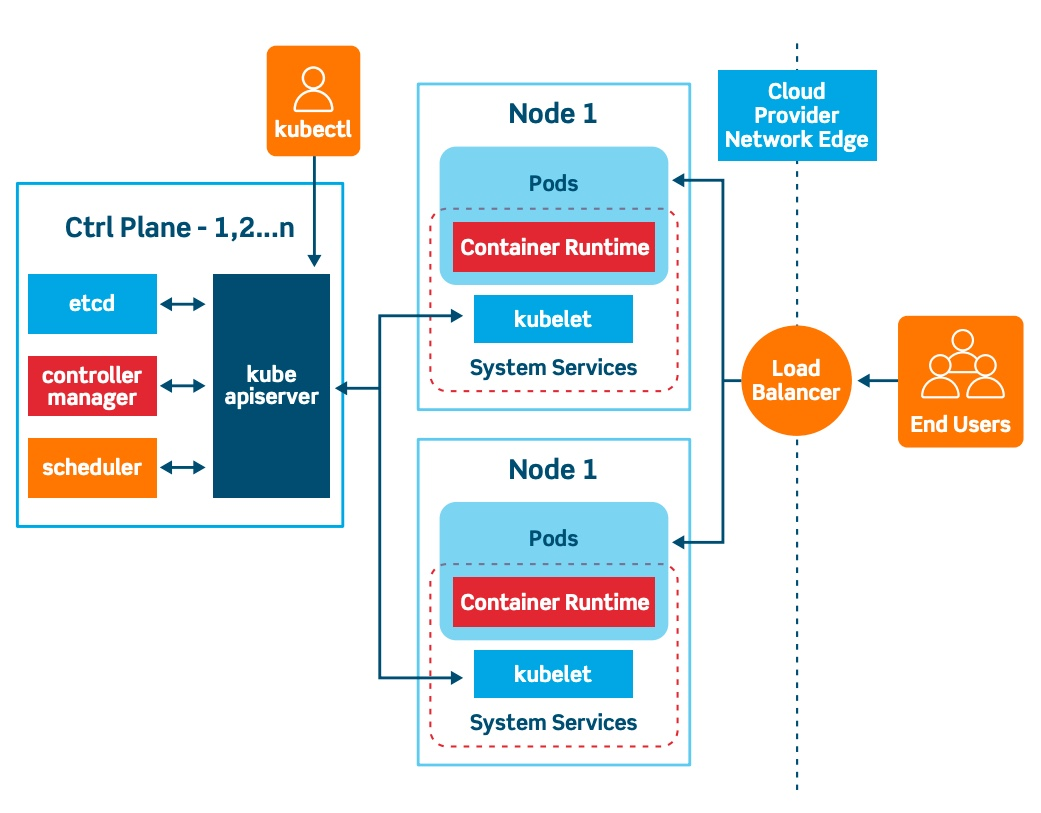
\includegraphics[width=400px]{figures/ch3/kube-arch.jpg}
    \caption[Architettura di un cluster Kubernetes]{Architettura di un cluster Kubernetes}
    \label{fig:cha3:k8s}
\end{figure}

\begin{itemize}
    \item \textbf{Master Node}:
    Il componente principale è il kube-apiserver, che fornisce l'interfaccia RESTful per l'interazione con il cluster. Tutte le operazioni di gestione sono effettuate attraverso questa API.
    Il etcd è uno storage persistente distribuito che memorizza lo stato del cluster, garantendo coerenza e disponibilità. È utilizzato come back-end per il kube-apiserver.
    Il kube-scheduler è responsabile della pianificazione dei pod su nodi disponibili, considerando i requisiti di risorse e le politiche di allocazione definite.

    \item \textbf{Node} (o Minion):
        Il componente fondamentale su ciascun nodo è il kubelet, che si occupa di mantenere l'integrità e l'esecuzione dei pod. Riceve istruzioni dal kube-apiserver per creare, aggiornare o rimuovere i pod sul nodo.
        Il kube-proxy gestisce il networking su ciascun nodo, facilitando la comunicazione tra i pod e consentendo l'esposizione dei servizi.
        Il Container Runtime è il software responsabile dell'esecuzione dei container. Docker è uno degli esempi più comuni di runtime supportati da Kubernetes, ma è possibile integrare altri come containerd o CRI-O.

    \item \textbf{Controller Manager}:
        Il kube-controller-manager ospita vari controller che monitorano continuamente lo stato del cluster e prendono azioni correttive quando necessario. Alcuni esempi includono il ReplicaSet Controller, il Deployment Controller e il StatefulSet Controller.

    \item \textbf{Cloud Controller Manager}:
        Il cloud-controller-manager delega specifiche funzionalità del provider cloud, come l'integrazione con load balancer o la gestione delle risorse, ad un controller specifico per ciascun provider cloud. Questo componente è opzionale e dipende dalla presenza di un ambiente cloud specifico.

    \item \textbf{Add-ons}:
        Kubernetes supporta vari add-on che estendono la funzionalità del cluster. Ad esempio, DNS facilita la risoluzione dei nomi all'interno del cluster, mentre Dashboard fornisce un'interfaccia web per la gestione del cluster.
\end{itemize}

Questa architettura fornisce una base solida per la creazione e la gestione di applicazioni distribuite su larga scala. La separazione dei ruoli e dei compiti tra i componenti, insieme alla comunicazione attraverso l'API server, consente una gestione efficiente e scalabile dei container su nodi multipli.

Sviluppare in locale su un cluster Kubernets, invece, richiede in genere l'impiego di strumenti terzi, come Minikube o Kind.


\subsubsection{Operare su un cluster Kind}

\glsname{kind} (Kubernetes In Docker) è uno strumento progettato per semplificare lo sviluppo locale su Kubernetes, consentendo agli sviluppatori di eseguire cluster Kubernetes completamente funzionali all'interno di container Docker. Questo approccio facilita il test e la validazione delle applicazioni in un ambiente controllato e isolato, simulando l'ambiente di produzione senza la necessità di infrastrutture complesse. L'approccio di Kind è particolarmente utile per gli sviluppatori che lavorano su applicazioni basate su microservizi o architetture a container.

La struttura di Kind si basa su container Docker leggeri, chiamati "node", ciascuno dei quali rappresenta un nodo nel cluster Kubernetes locale. Ogni nodo viene eseguito come un container Docker separato, consentendo la creazione rapida e la distruzione dei cluster Kubernetes all'interno dell'ambiente di sviluppo dell'utente.

Il processo di sviluppo locale su Kubernetes con Kind comprende diversi passaggi chiave:

L'utente installa Kind sulla propria macchina locale, seguendo le istruzioni specificate nella documentazione ufficiale. Kind è progettato per essere facilmente installabile attraverso strumenti come Homebrew o direttamente da GitHub.

\begin{figure}[h]
    \centering
    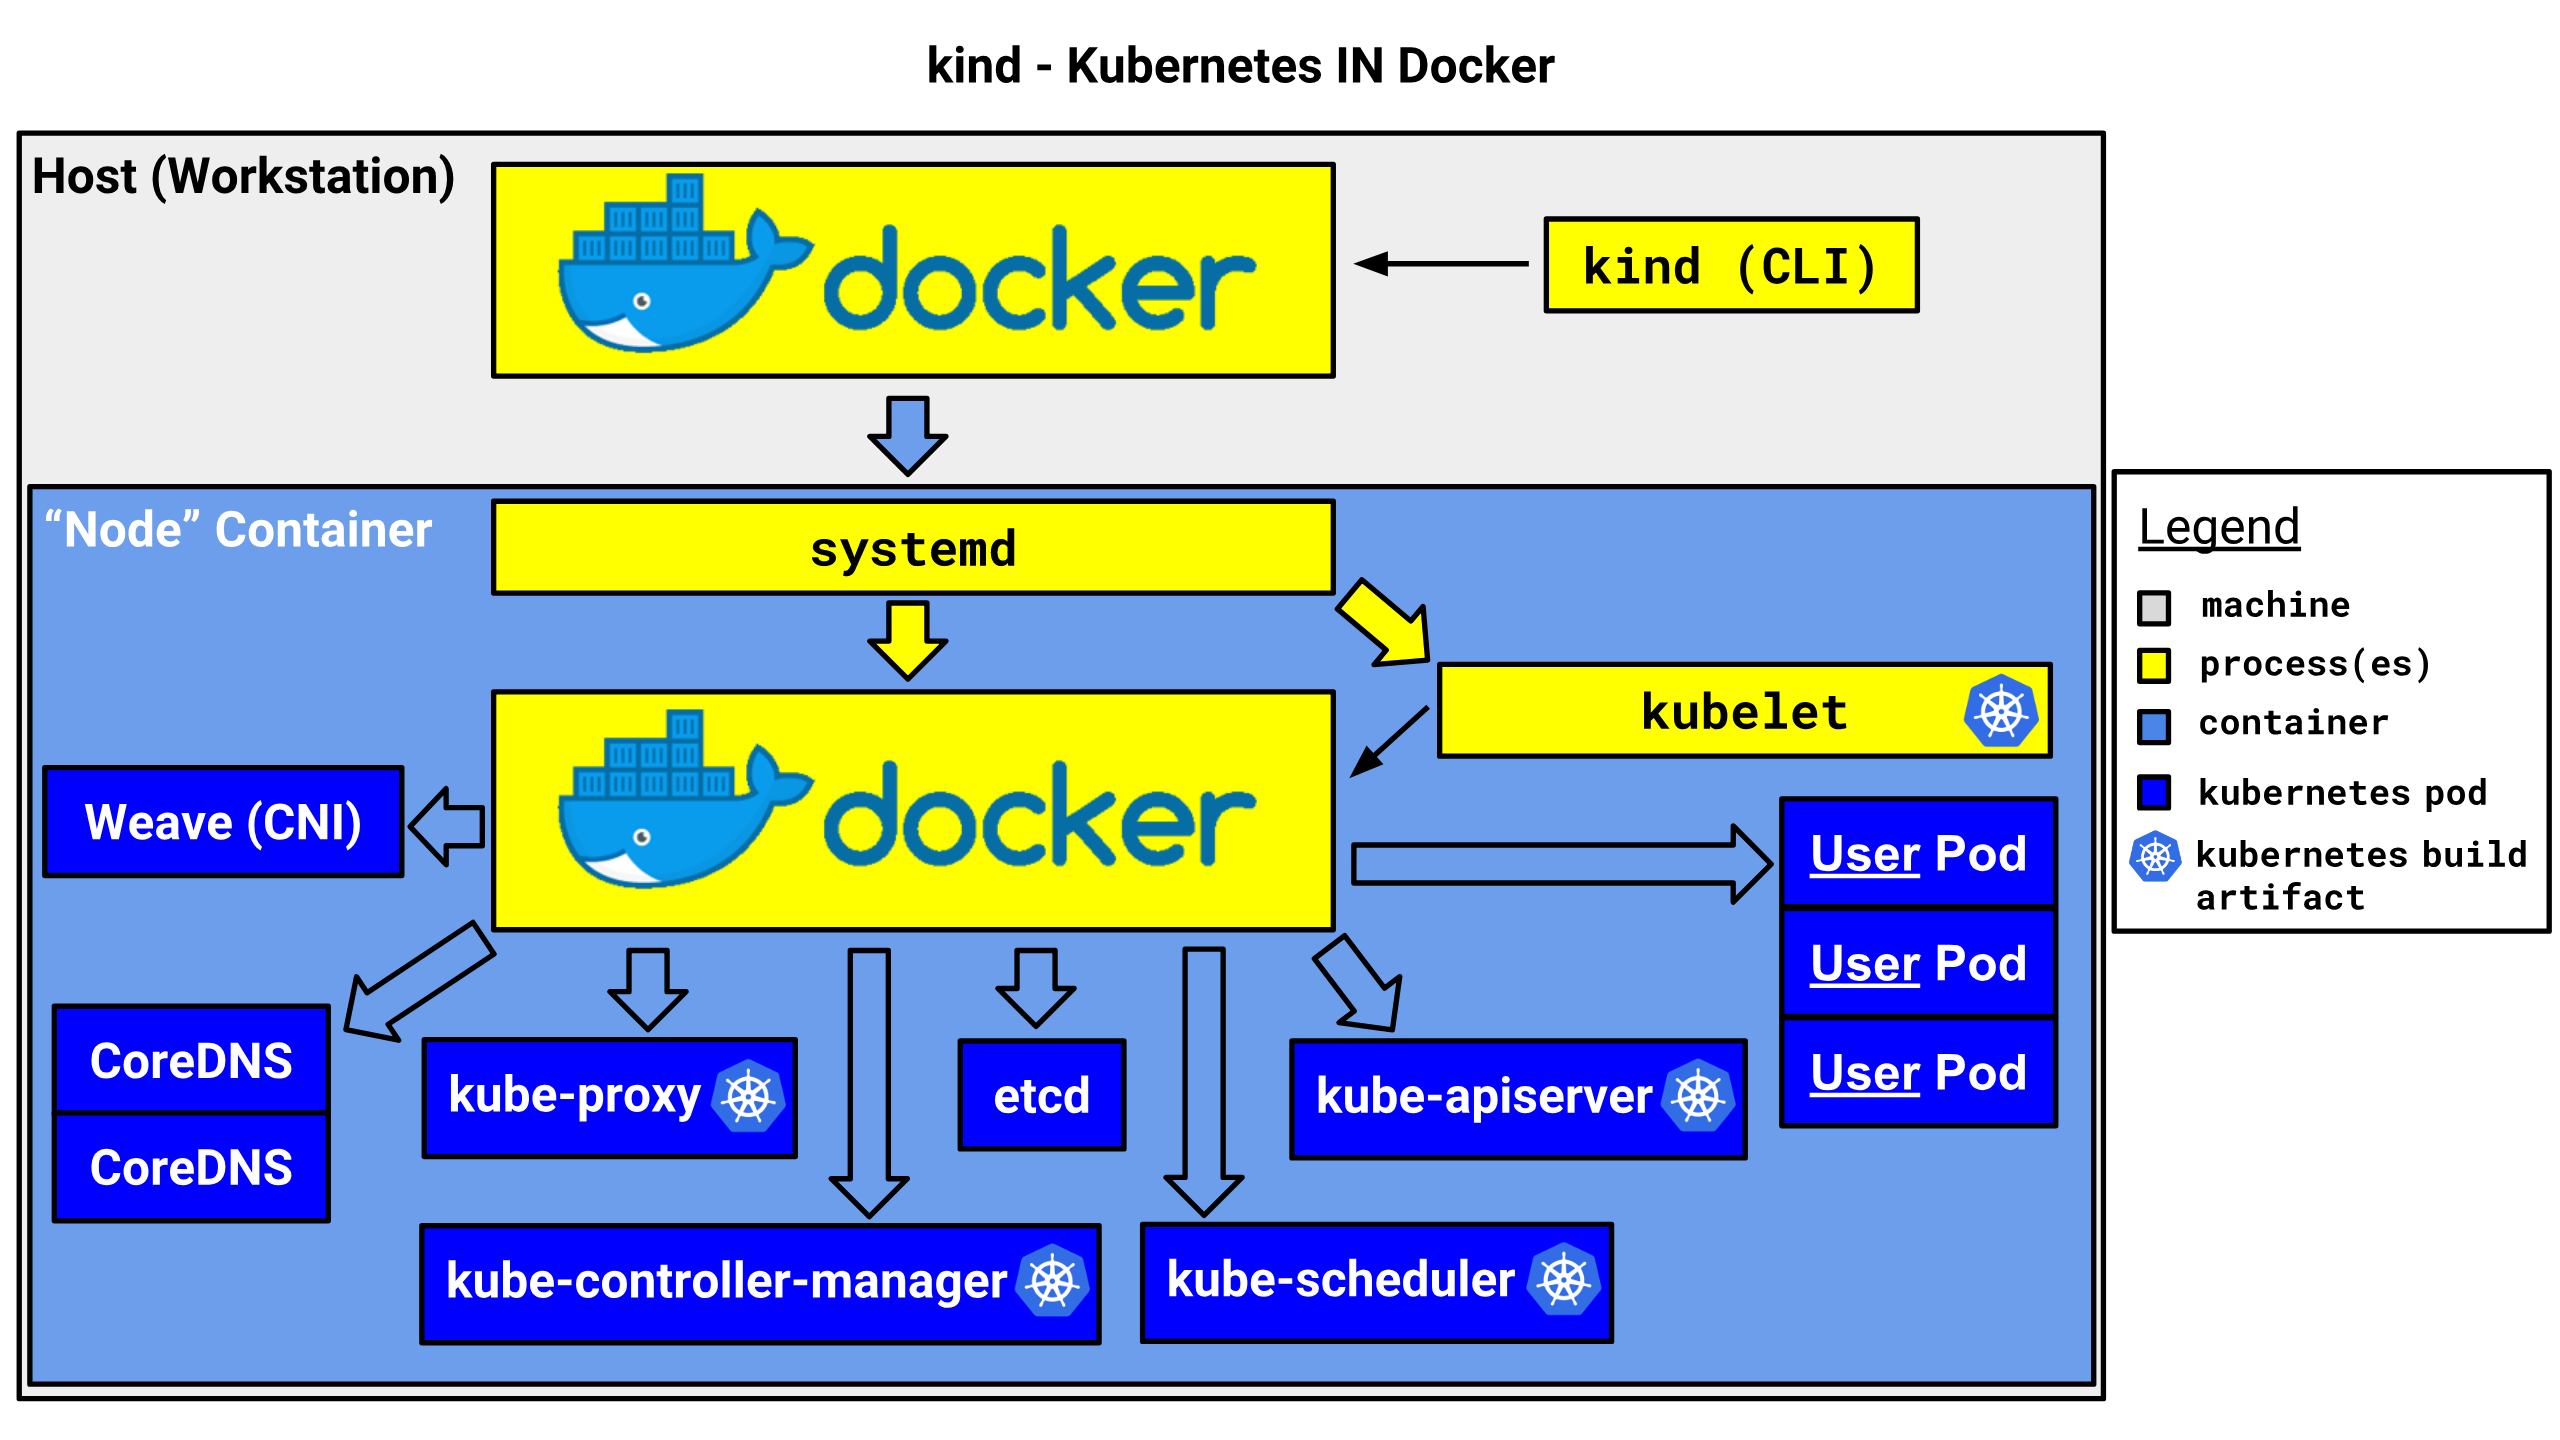
\includegraphics[width=\linewidth]{figures/ch3/kind.png}
    \caption[Architettura di un cluster Kind]{Architettura di un cluster Kind}
    \label{fig:cha3:kind}
\end{figure}

Una volta installato, l'utente può creare un cluster Kubernetes locale eseguendo un comando specifico di Kind. Questo comando avvia i container Docker che fungono da nodi Kubernetes, creando un cluster completamente funzionale. Kind offre opzioni di configurazione per personalizzare il comportamento del cluster. Gli utenti possono specificare la versione di Kubernetes, il numero di nodi, e altre opzioni secondo le esigenze del loro sviluppo.

L'utente può interagire con esso utilizzando le normali operazioni di Kubernetes come {\small \verb|kubectl|}. Ciò consente agli sviluppatori di distribuire, gestire e monitorare le proprie applicazioni come farebbero in un ambiente di produzione Kubernetes.

L'approccio di Kind si basa sulla facilità d'uso e sulla portabilità, fornendo uno strumento agile per lo sviluppo su Kubernetes. L'utilizzo di container Docker come nodi del cluster consente di risparmiare risorse rispetto alla creazione di macchine virtuali separate per ciascun nodo, rendendo il processo più veloce ed efficiente.

In conclusione, l'adozione di Kind nell'ecosistema Kubernetes offre un modo efficiente per sviluppare, testare e validare applicazioni in un ambiente locale controllato, contribuendo a migliorare la produttività degli sviluppatori e garantendo una coerenza tra gli ambienti di sviluppo e produzione.

\clearpage